\section{5. Entregables}

\subsection{Tablero Kanban Activo}
El tablero Kanban se encuentra 100\% operativo y poblado en la plataforma oficial de Jira Software:
\begin{center}
    \url{https://unsaac-team-grupois.atlassian.net/jira/software/projects/SC/boards/136}
\end{center}

Los requerimientos gestionados en este tablero provienen directamente del acta de validación formal sostenida el 20 de octubre de 2026 entre \textbf{Franklin Choquenaira} y el \textbf{Lic. Adrian Valer}, Director de la Oficina de Tecnologías de la Información (OTI) de la Municipalidad Distrital de San Jerónimo:

\begin{figure}[H]
    \centering
    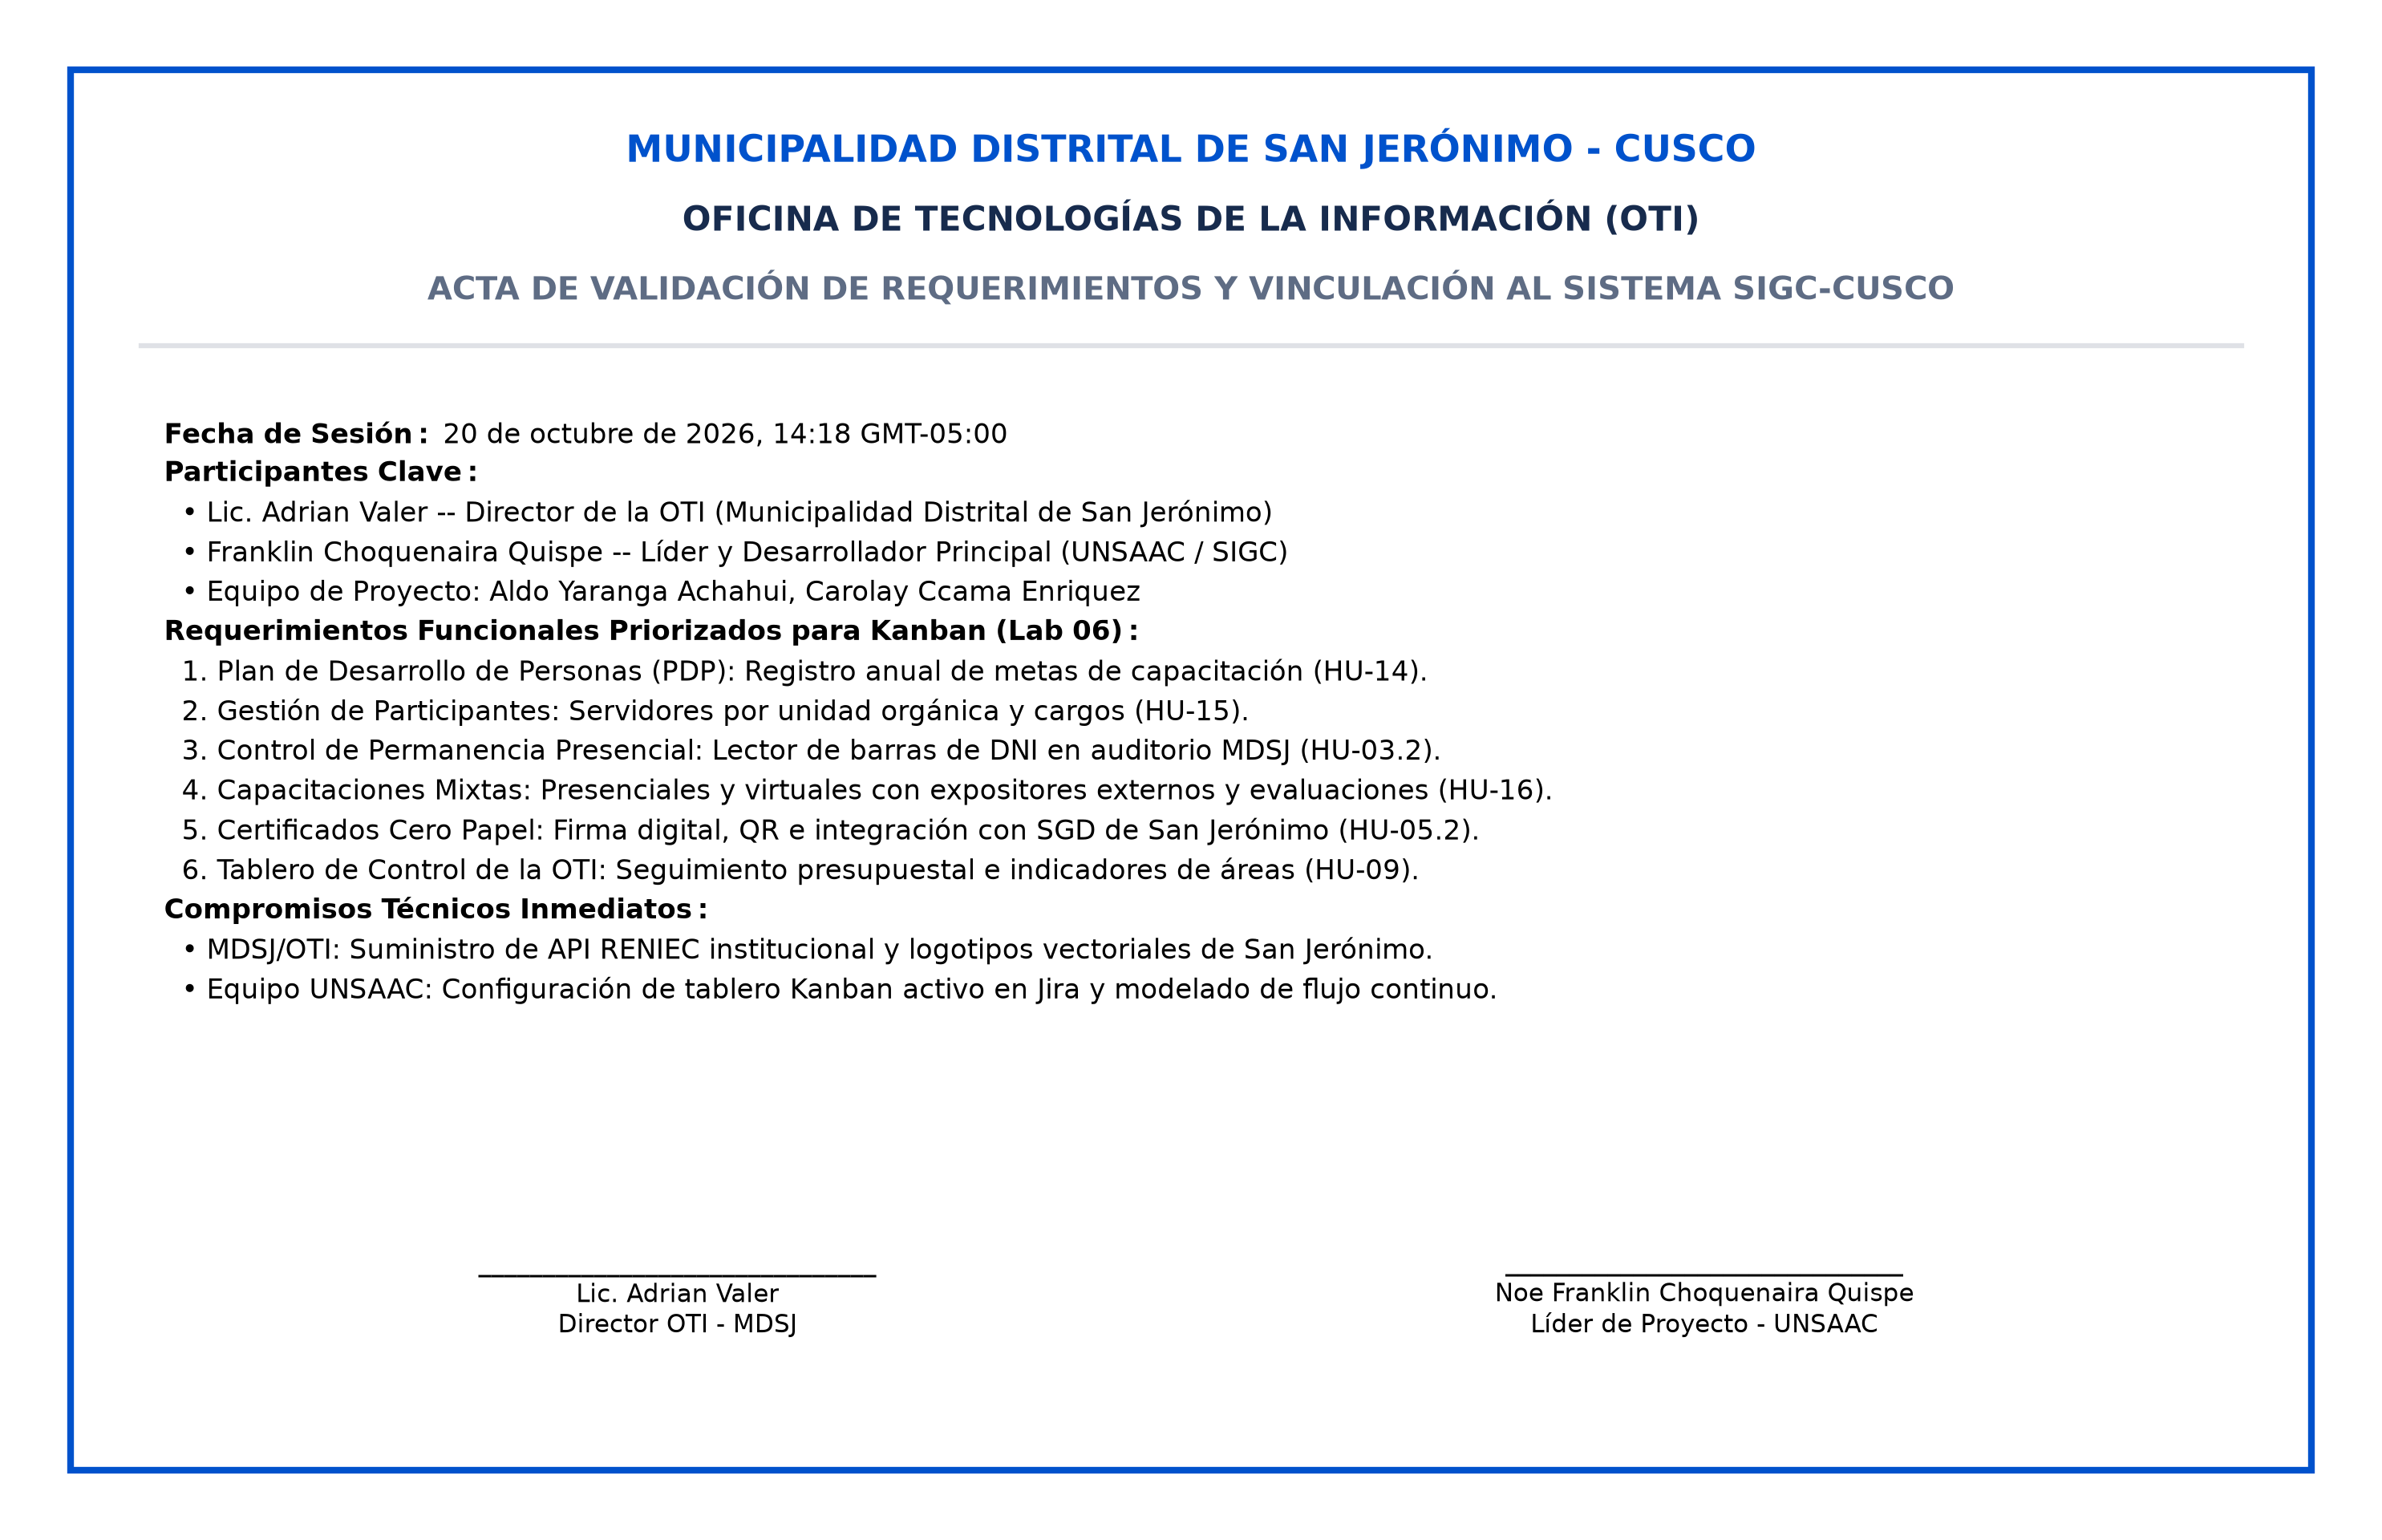
\includegraphics[width=0.88\textwidth]{captura_acta_reunion_mdsj.png}
    \caption{Acta Oficial de Validación de Requerimientos con la Municipalidad Distrital de San Jerónimo.}
    \label{fig:acta_mdsj}
\end{figure}

\subsection{Historias Distribuidas Correctamente}
El inventario de 41 incidencias del proyecto SIGC-CUSCO se encuentra distribuido de forma balanceada:

\begin{table}[H]
\centering
\small
\caption{Distribución Actual de Historias en el Tablero de Jira.}
\label{tab:distribucion}
\begin{tabularx}{\textwidth}{P{2.5cm} P{1.8cm} Y}
\toprule
\textbf{Estado} & \textbf{Cantidad} & \textbf{Historias y Módulos Representativos} \\
\midrule
\textbf{Por hacer} & 32 tareas & \texttt{SC-44} (Spike RENIEC MDSJ), \texttt{SC-24} (Dashboard PDP), \texttt{SC-13} (Usuarios y roles), \texttt{SC-18} (Login DNI), \texttt{SC-26} (Catálogo público), \texttt{SC-42} (Servidores por área). \\
\addlinespace[0.1cm]
\textbf{En progreso} & \textbf{3 tareas} & \texttt{SC-35} (Certificado virtual firma/QR -- Franki), \texttt{SC-32} (Lector DNI auditorio -- Aldo), \texttt{SC-41} (Registro anual PDP -- Carolay). \textbf{WIP = 3/3 cumplido.} \\
\addlinespace[0.1cm]
\textbf{En revisión} & \textbf{0 tareas} & Capacidad disponible (WIP máx: 2). \\
\addlinespace[0.1cm]
\textbf{Terminado} & 6 tareas & \texttt{SC-19} (Inscripción con DNI) y módulos base \texttt{SC-02} a \texttt{SC-06}. \\
\bottomrule
\end{tabularx}
\end{table}

\subsection{Métricas Básicas de Flujo}
El comportamiento del sistema fue auditado cuantitativamente mediante el Diagrama de Flujo Acumulado (CFD) y el análisis de tiempos de entrega:

\begin{figure}[H]
    \centering
    \begin{subfigure}[b]{0.48\textwidth}
        \centering
        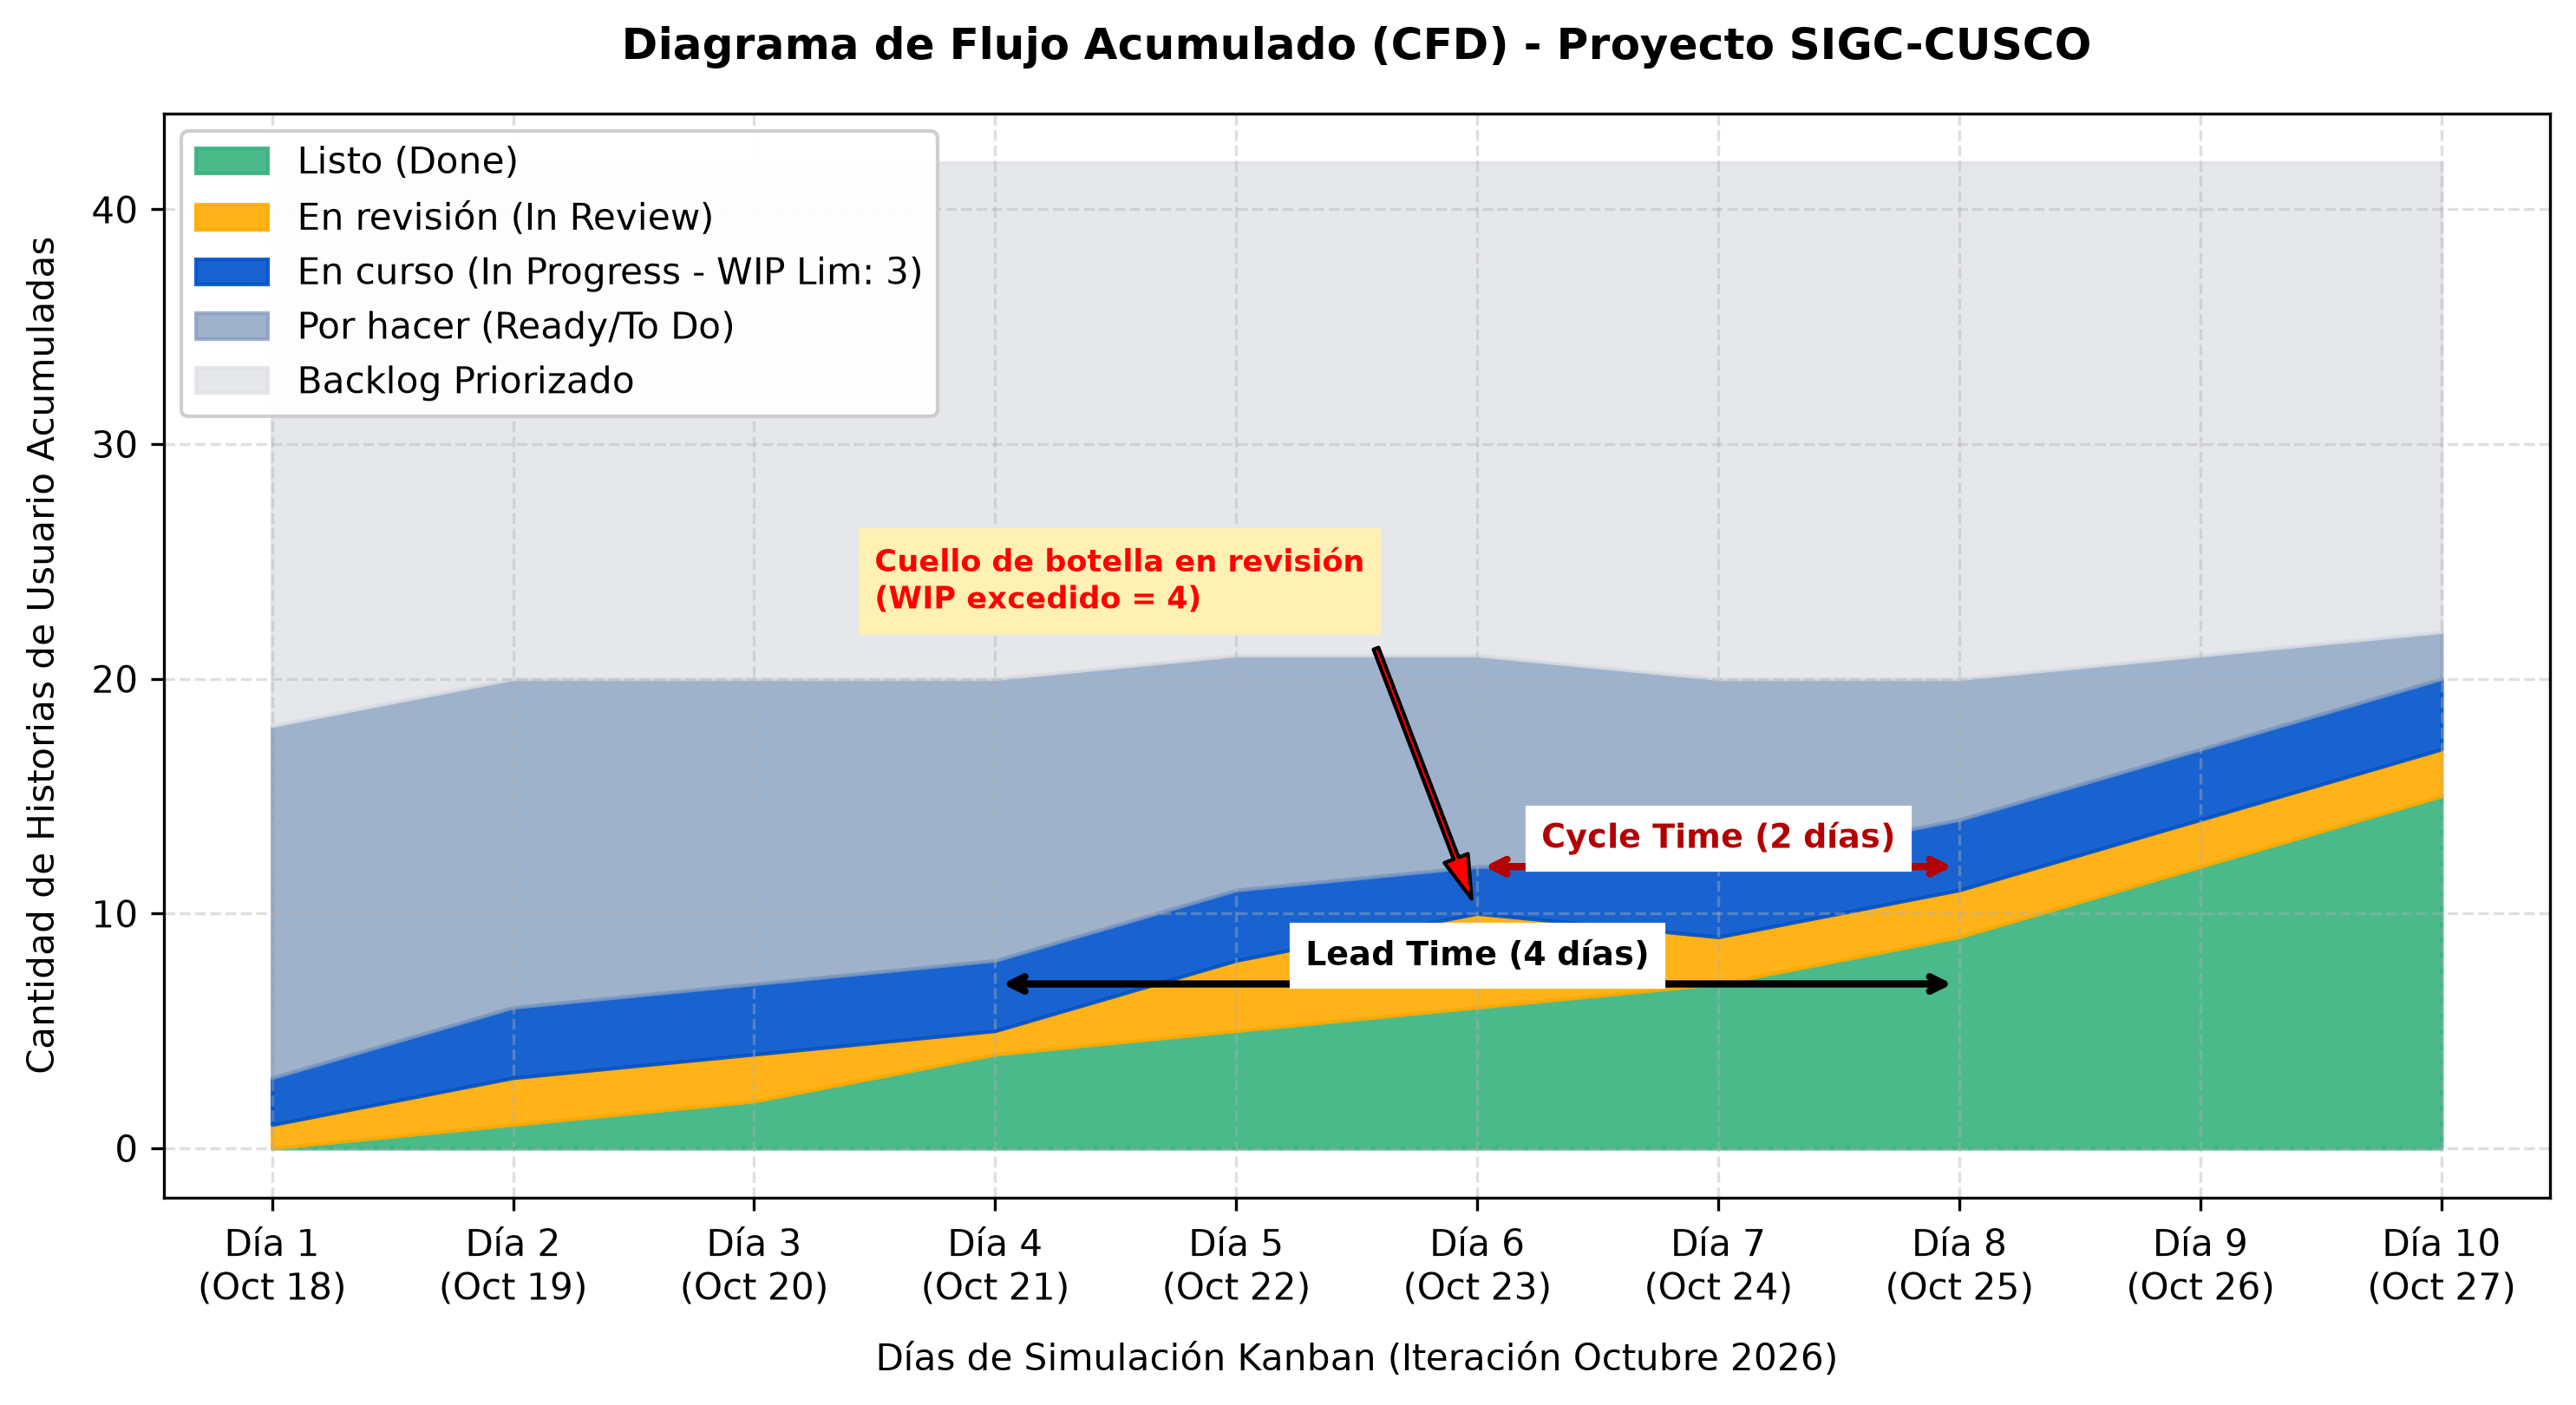
\includegraphics[width=\textwidth]{captura_cfd_diagrama_flujo.png}
        \caption{Diagrama de Flujo Acumulado (CFD).}
    \end{subfigure}
    \hfill
    \begin{subfigure}[b]{0.48\textwidth}
        \centering
        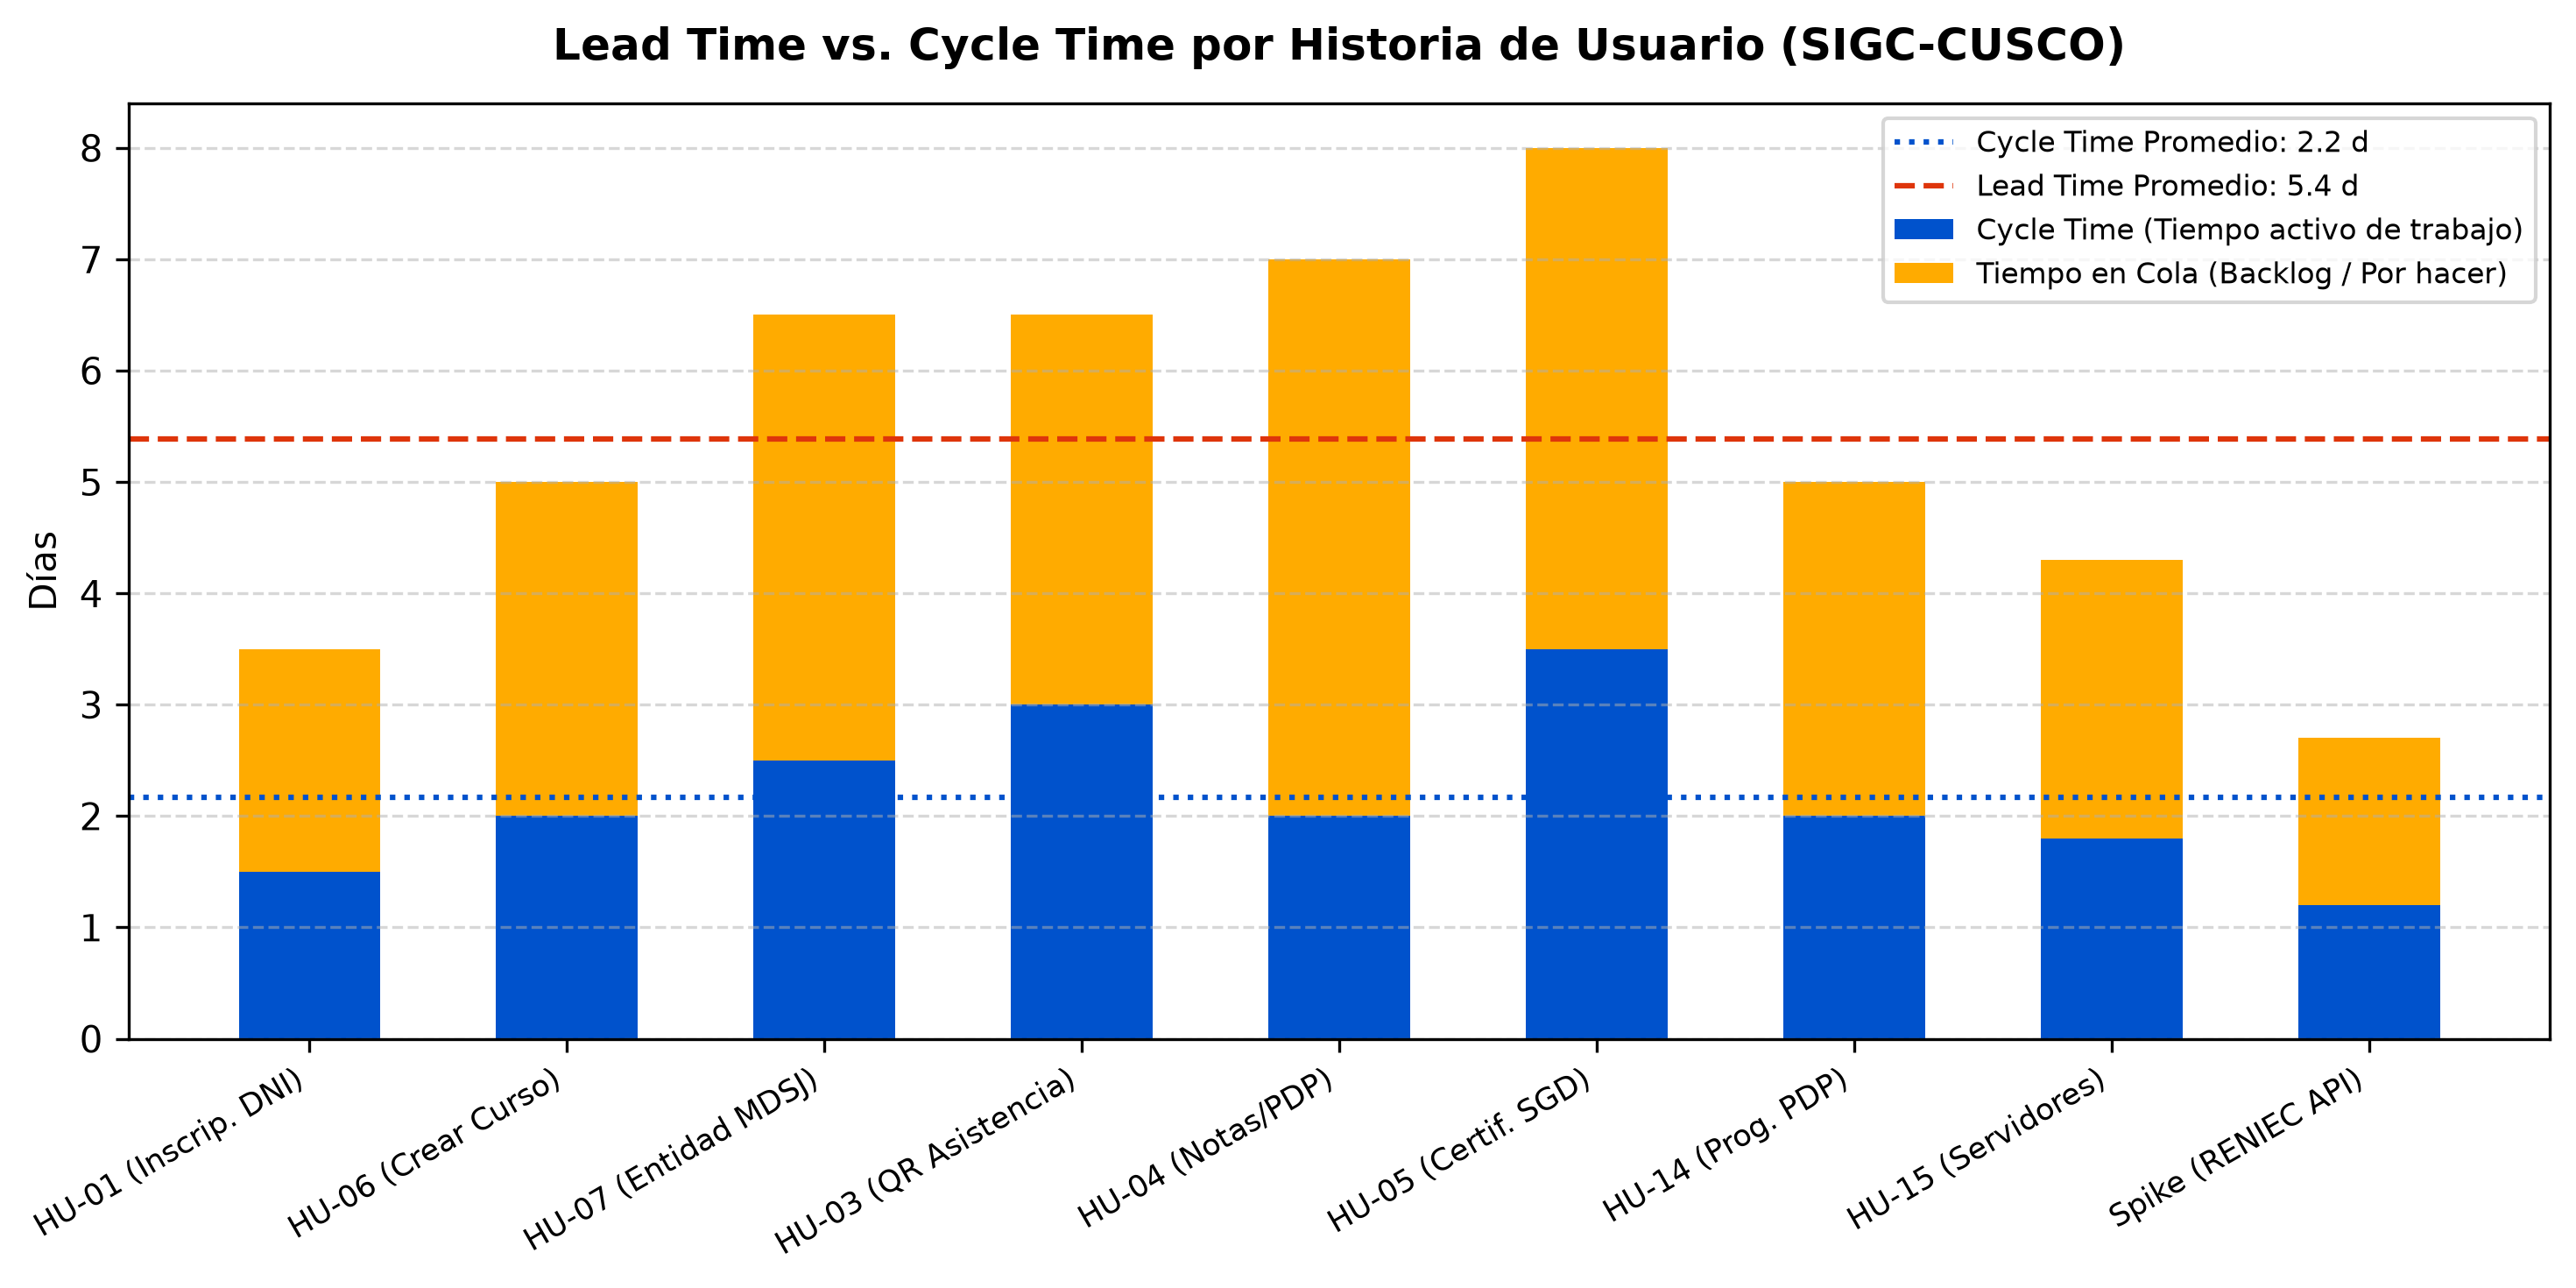
\includegraphics[width=\textwidth]{captura_lead_cycle_time.png}
        \caption{Lead Time vs. Cycle Time por Historia.}
    \end{subfigure}
    \caption{Métricas Cuantitativas de Flujo del Proyecto SIGC-CUSCO.}
    \label{fig:metricas}
\end{figure}

\begin{table}[H]
\centering
\small
\caption{Resumen de Métricas de Flujo en Estado Estable.}
\label{tab:metricas_resumen}
\begin{tabularx}{\textwidth}{P{3.5cm} P{2.5cm} Y}
\toprule
\textbf{Métrica} & \textbf{Valor Medido} & \textbf{Interpretación Técnica en el Proyecto} \\
\midrule
\textbf{Throughput Promedio} & 1.5 historias/día & Ritmo constante de entrega del equipo de desarrollo. \\
\textbf{Cycle Time Promedio} & 2.10 días & Tiempo neto desde que se empieza a programar hasta que se termina. \\
\textbf{Lead Time Promedio} & 5.02 días & Tiempo total desde la priorización del requerimiento en la MDSJ. \\
\bottomrule
\end{tabularx}
\end{table}

\noindent\textbf{Comprobación de la Ley de Little:}
\begin{equation}
    \text{Cycle Time Teórico} = \frac{\text{WIP}}{\text{Throughput}} = \frac{5 \text{ historias}}{1.5 \text{ historias/día}} = 3.33 \text{ días}
\end{equation}
El valor experimental obtenido (promedio de 2.10 días) corrobora que mantener el WIP total $\le 5$ asegura entregas en menos de 3.5 días laborables.

\subsection{Evidencias de Implementación del Sistema SIGC-CUSCO}
El flujo modelado en Jira corresponde a módulos de software reales desarrollados en el repositorio \texttt{SIGC-CUSCO}:

\begin{figure}[H]
    \centering
    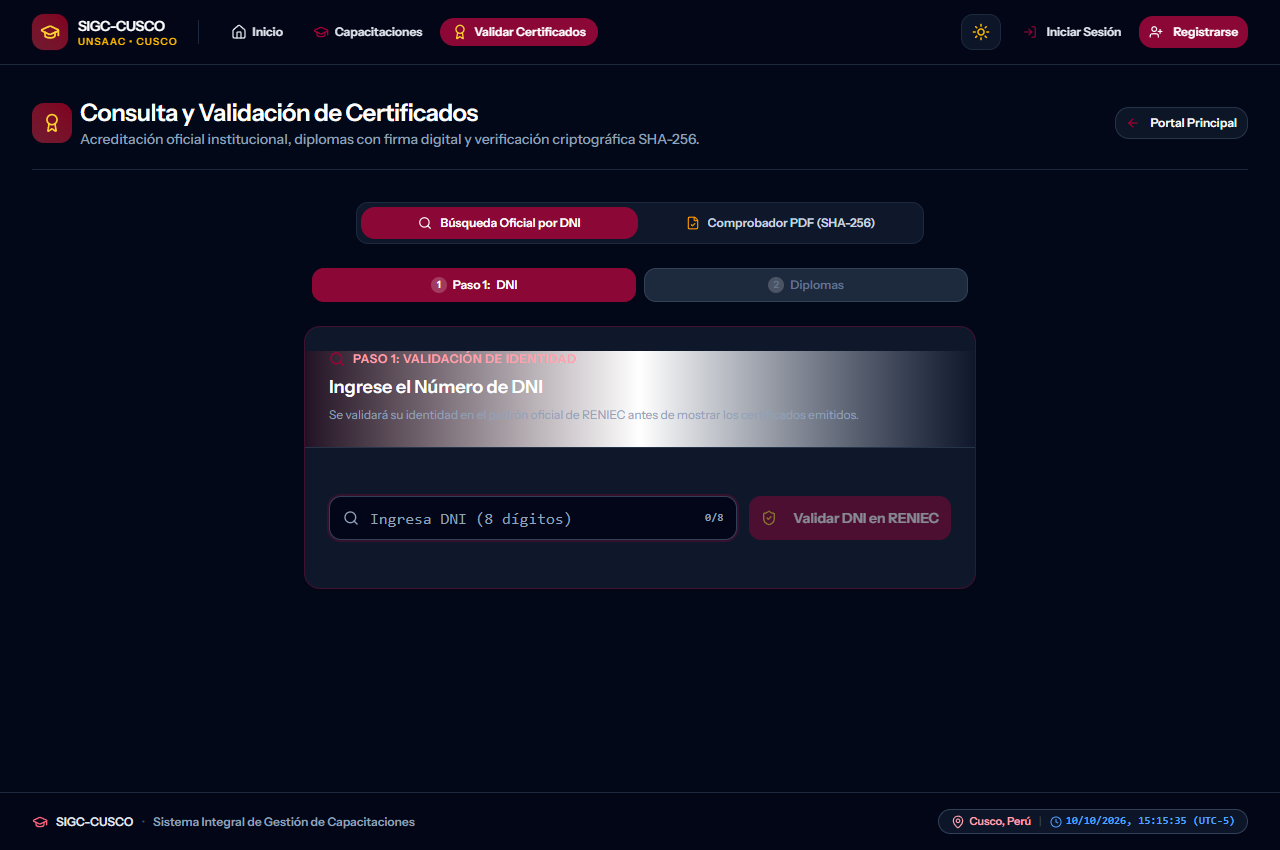
\includegraphics[width=0.85\textwidth]{captura_certificados.png}
    \caption{Módulo de Emisión y Validación QR de Certificados Digitales (\textit{SC-35 y SC-22}).}
    \label{fig:evidencia_certificados}
\end{figure}

\begin{figure}[H]
    \centering
    \begin{subfigure}[b]{0.48\textwidth}
        \centering
        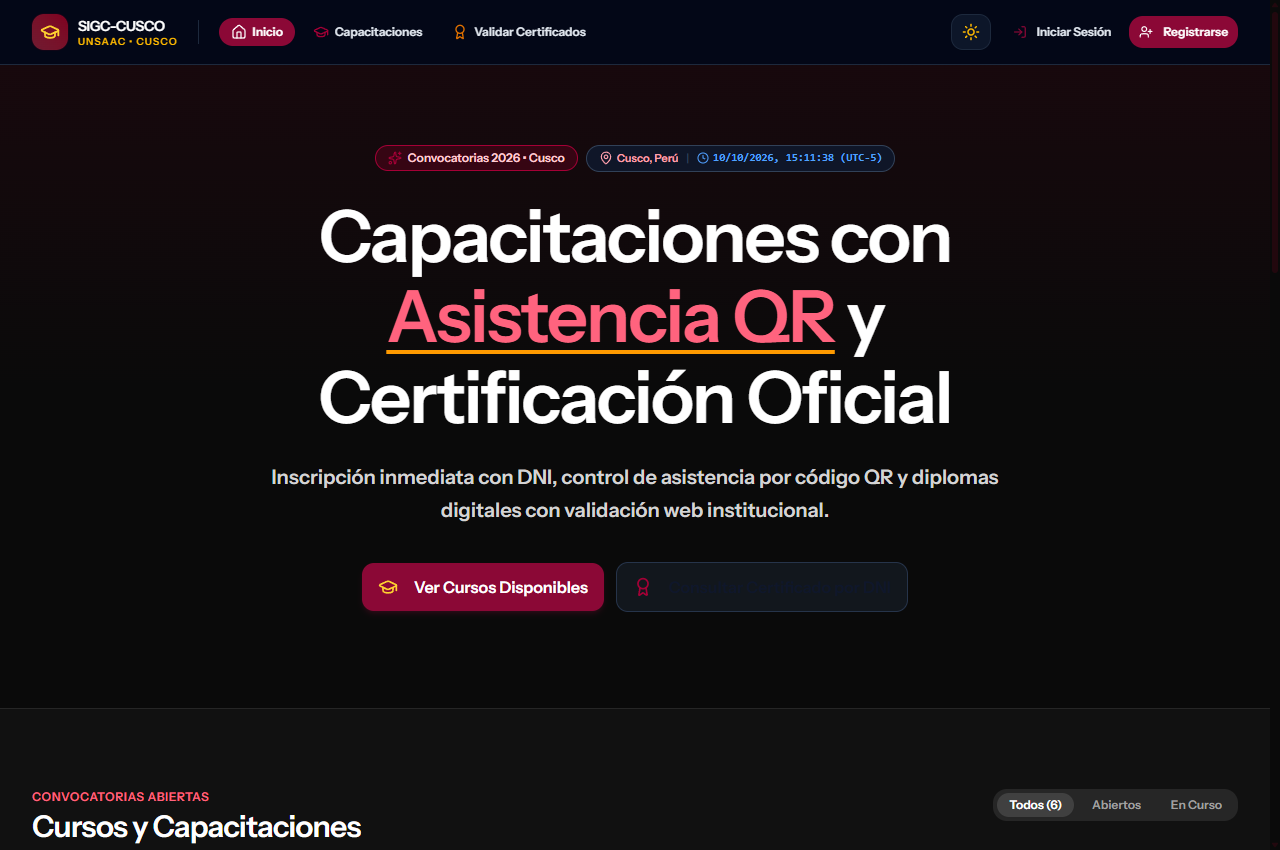
\includegraphics[width=\textwidth]{captura_catalogo.png}
        \caption{Catálogo de Capacitaciones (\textit{SC-26}).}
    \end{subfigure}
    \hfill
    \begin{subfigure}[b]{0.48\textwidth}
        \centering
        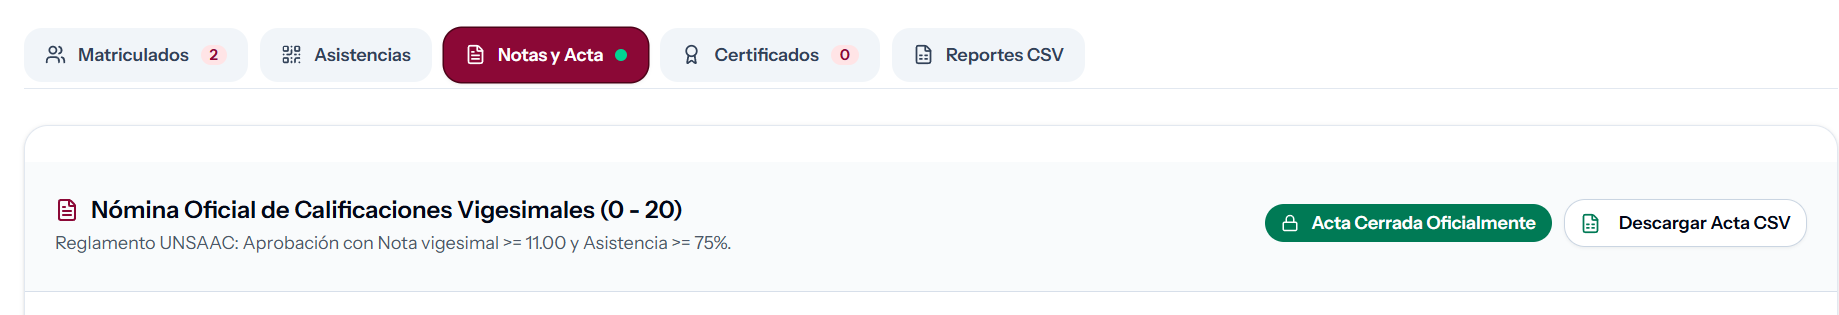
\includegraphics[width=\textwidth]{captura_nomina_acta.png}
        \caption{Nómina y Asistencia de Servidores (\textit{SC-32}).}
    \end{subfigure}
    \caption{Vistas del Catálogo y Control de Asistencia para la Municipalidad de San Jerónimo.}
    \label{fig:evidencias_ui}
\end{figure}
